\documentclass{article}
\usepackage[a4paper, total={7in, 9.5in}]{geometry}
\usepackage{amsmath,amsfonts,amsthm,amssymb,graphicx,float, setspace, bm}
\usepackage[utf8]{inputenc}
\usepackage{float}
\usepackage{titlesec}
\usepackage{setspace}
\usepackage{geometry}
\usepackage[style=numeric]{biblatex}
\usepackage[autostyle=true]{csquotes}
\usepackage{breqn}
\usepackage{subfig}
\usepackage[bottom]{footmisc}
\usepackage{adjustbox}
\usepackage{lipsum}
\usepackage{hyperref}
\usepackage[ruled,vlined]{algorithm2e}
\hypersetup{
    colorlinks=true,
    urlcolor=magenta
}
\usepackage[table,x11names]{xcolor}

\usepackage{xltabular}
\usepackage{multirow}
\usepackage{booktabs}


\renewcommand{\baselinestretch}{1.5} 
\setlength\parindent{0pt}
%----------------------------------------------------------------------------------------
%	START
%----------------------------------------------------------------------------------------

\newcommand{\horrule}[1]{\rule{\linewidth}{#1}}

\title{ \normalfont \normalsize 
\huge CPSC 532W - Homework 4}
\date{}
\author{Xiaoxuan Liang - 48131163}
\def\cond{\; | \;}

\begin{document}

\maketitle

Public GitHub repo: https://github.com/Xiaoxuan1121/CPSC532W/tree/main/a4
\begin{enumerate}
\item Program 1:

\begin{figure}[!ht]
	\centering
	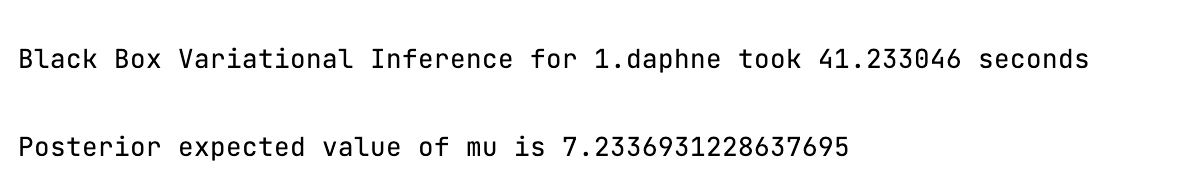
\includegraphics[scale=0.5]{../figs/1_daphne_results}
\end{figure}

\begin{figure}[!ht]
	\centering
	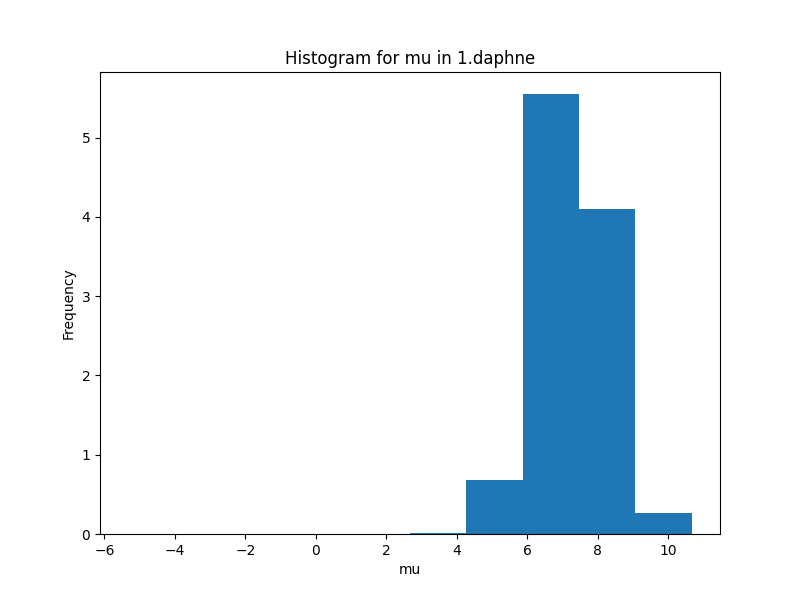
\includegraphics[scale=0.5]{../figs/1_daphne_histogram}
	\caption{Posterior distribution for mu for 1.daphne using Black Box Variational Inference}
\end{figure}

\begin{figure}[!ht]
	\centering
	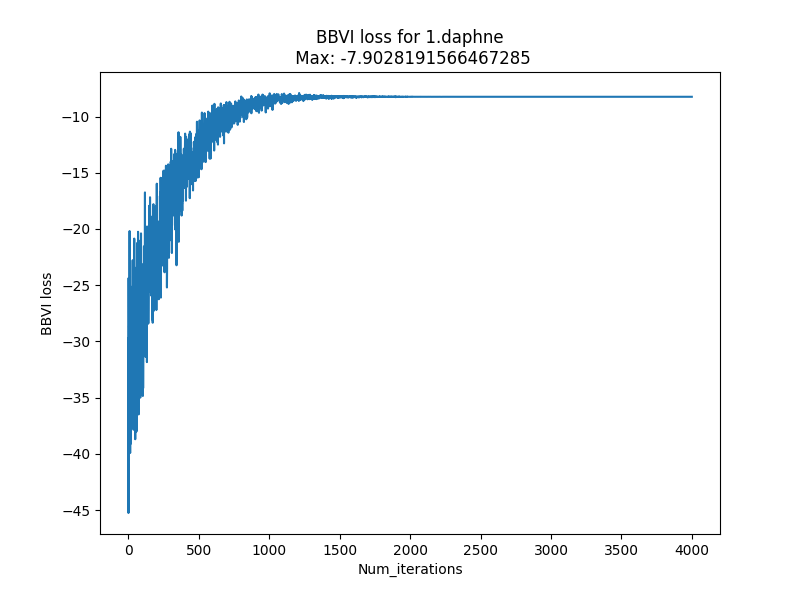
\includegraphics[scale=0.5]{../figs/1_daphne_ELBO}
	\caption{ELBO for 1.daphne}
\end{figure}

\newpage
\item Program 2:

\begin{figure}[!ht]
	\centering
	
\includegraphics[scale=0.5]{../figs/2_daphne_results}
\end{figure}


\begin{figure}[!htp] 
    \centering
    \subfloat[Samples from the posterior for slope]{%
        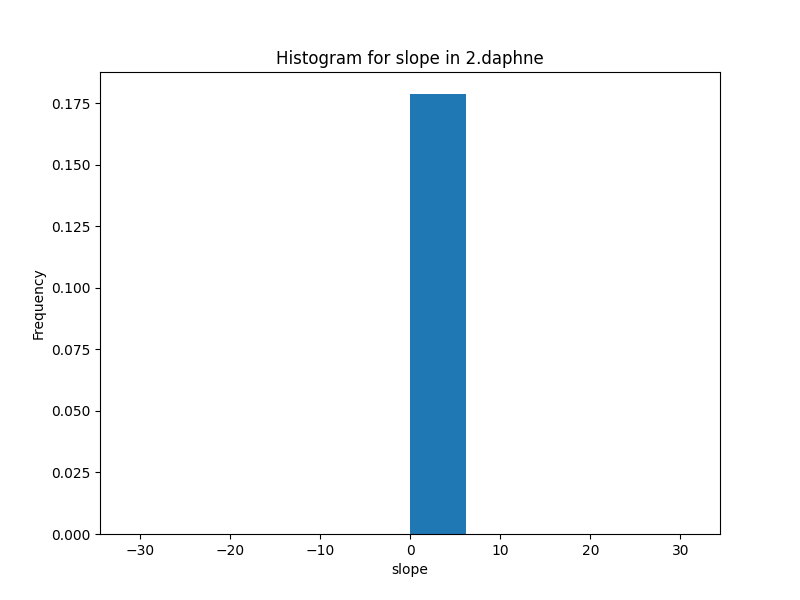
\includegraphics[width=0.5\textwidth]{../figs/2_daphne_slope_histogram}%
        \label{fig:a}%
        }%
    \hfill%
    \subfloat[Samples from the posterior for bias]{%
        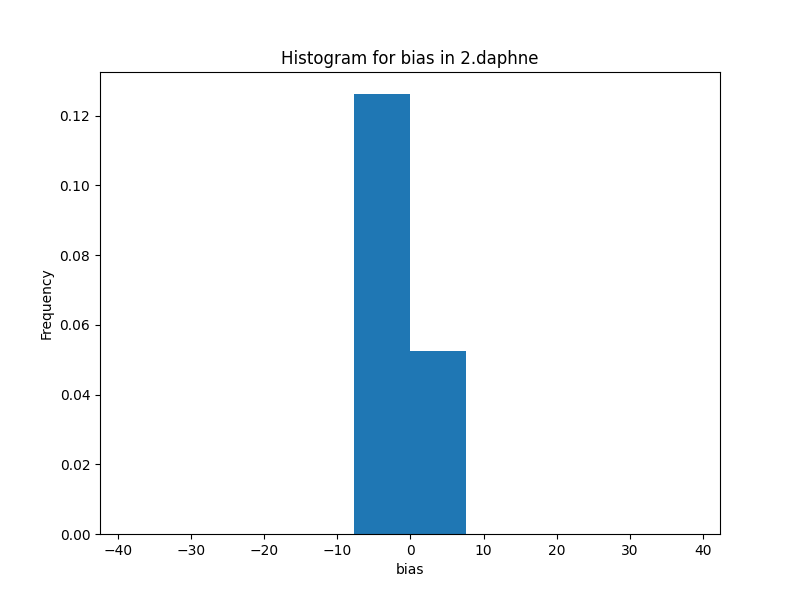
\includegraphics[width=0.5\textwidth]{../figs/2_daphne_bias_histogram}%%
        \label{fig:b}%
        }%
        \caption{Posterior distribution for slope and bias for 2.daphne using Black Box Variational Inference}
\end{figure}

\begin{figure}[!ht]
	\centering
	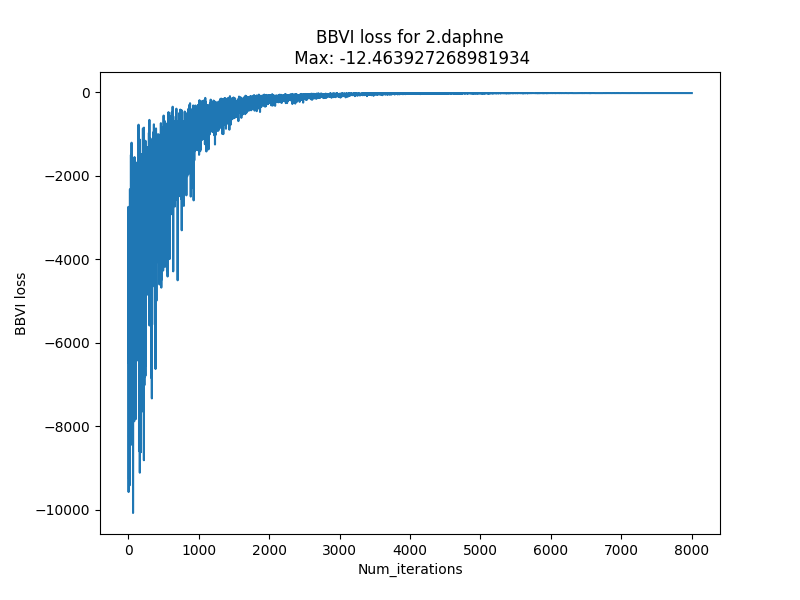
\includegraphics[scale=0.5]{../figs/2_daphne_ELBO}
	\caption{ELBO for 2.daphne}
\end{figure}

\newpage
\item  Program 3
\item  Program 4

\begin{figure}[!ht]
	\centering
	
\includegraphics[scale=0.5]{../figs/4_daphne_results}
\end{figure}

\begin{figure}[!ht]
	\centering
	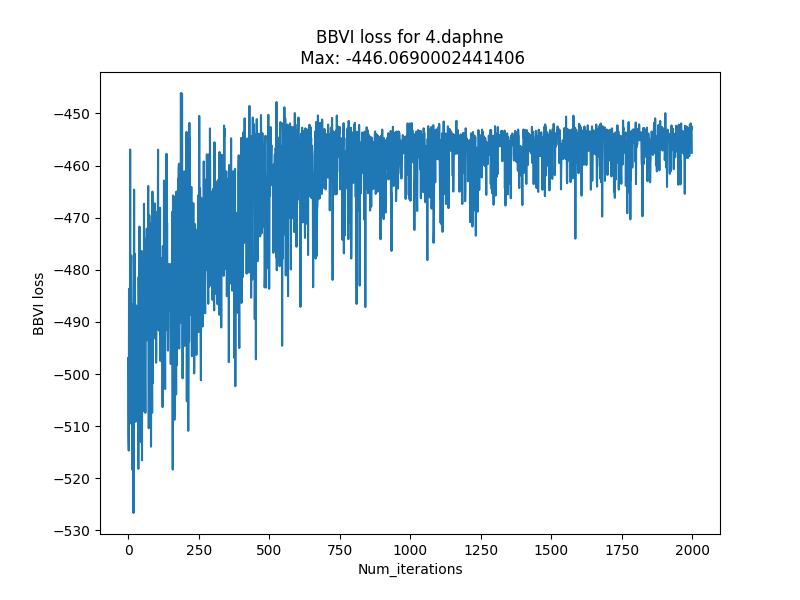
\includegraphics[scale=0.5]{../figs/4_daphne_ELBO}
	\caption{ELBO for 4.daphne}
\end{figure}

\begin{figure}[!htp] 
    \centering
    \subfloat[Samples from the posterior for slope]{%
        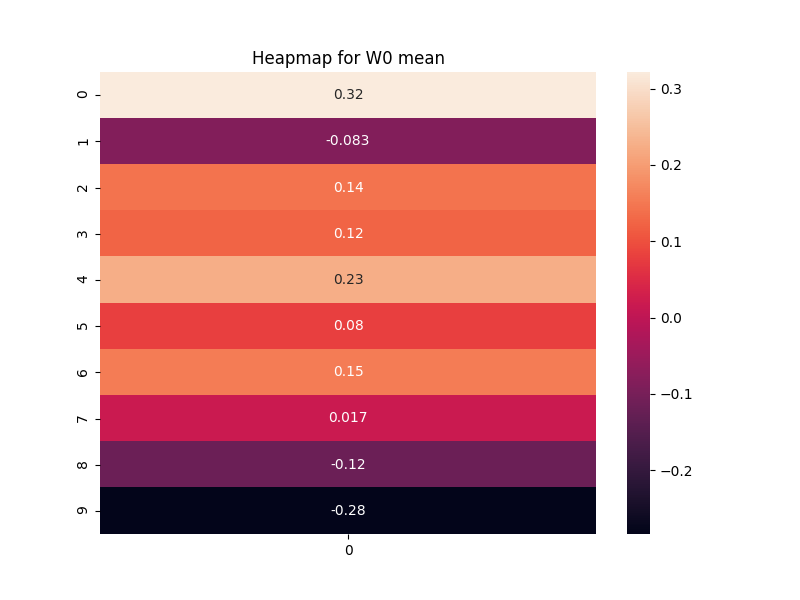
\includegraphics[width=0.5\textwidth]{../figs/4_daphne_w0_mean_heatmap.png}%
        \label{fig:a}%
        }%
    \hfill%
    \subfloat[Samples from the posterior for bias]{%
        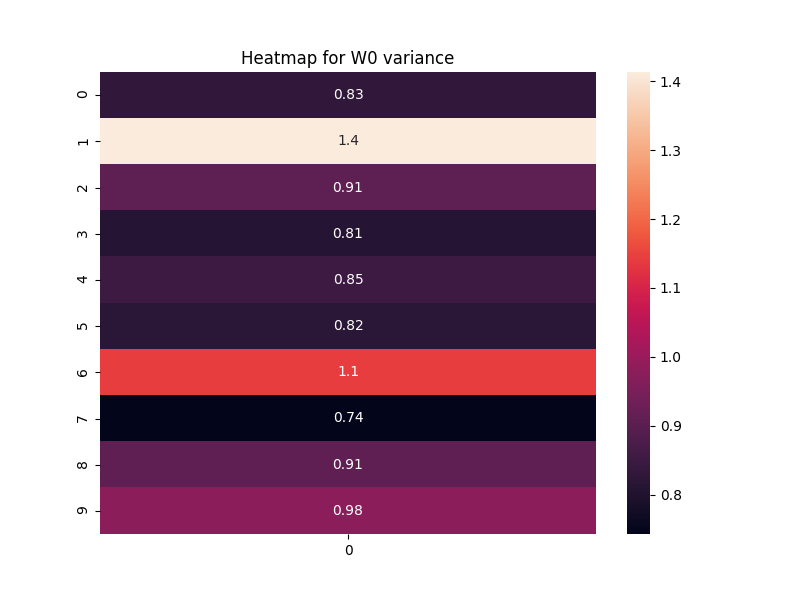
\includegraphics[width=0.5\textwidth]{../figs/4_daphne_w0_variance_heatmap.png}%%
        \label{fig:b}%
        }%
        \caption{Posterior distribution for slope and bias for 4.daphne using Black Box Variational Inference}
\end{figure}

\begin{figure}[!htp] 
    \centering
    \subfloat[Samples from the posterior for slope]{%
        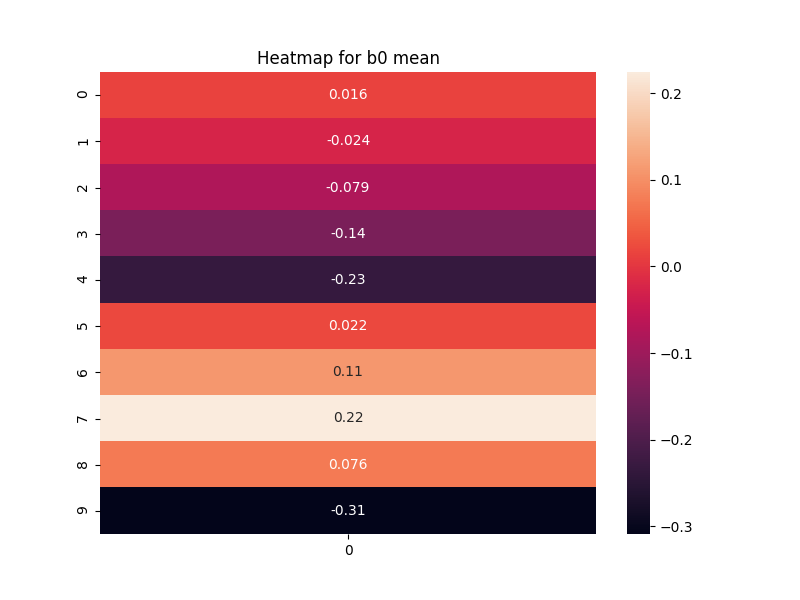
\includegraphics[width=0.5\textwidth]{../figs/4_daphne_b0_mean_heatmap.png}%
        \label{fig:a}%
        }%
    \hfill%
    \subfloat[Samples from the posterior for bias]{%
        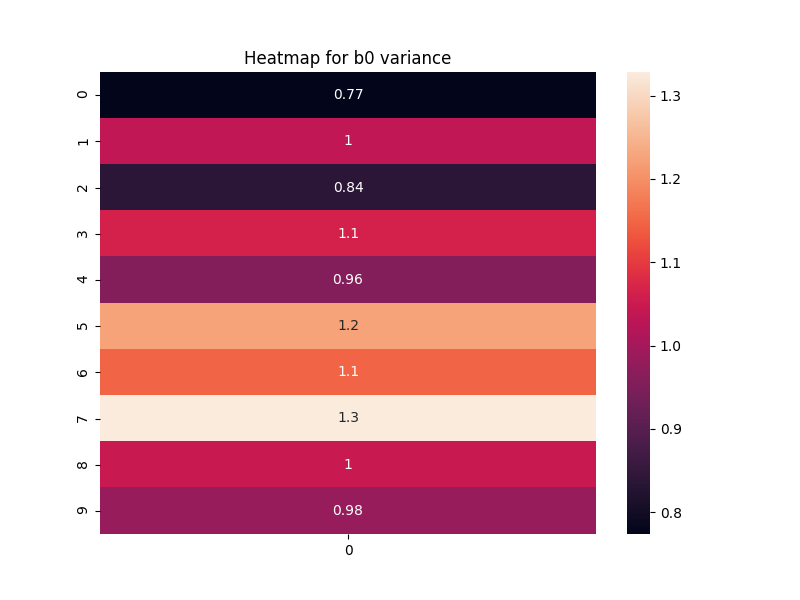
\includegraphics[width=0.5\textwidth]{../figs/4_daphne_b0_variance_heatmap.png}%%
        \label{fig:b}%
        }%
        \caption{Posterior distribution for slope and bias for 4.daphne using Black Box Variational Inference}
\end{figure}

\begin{figure}[!htp] 
    \centering
    \subfloat[Samples from the posterior for slope]{%
        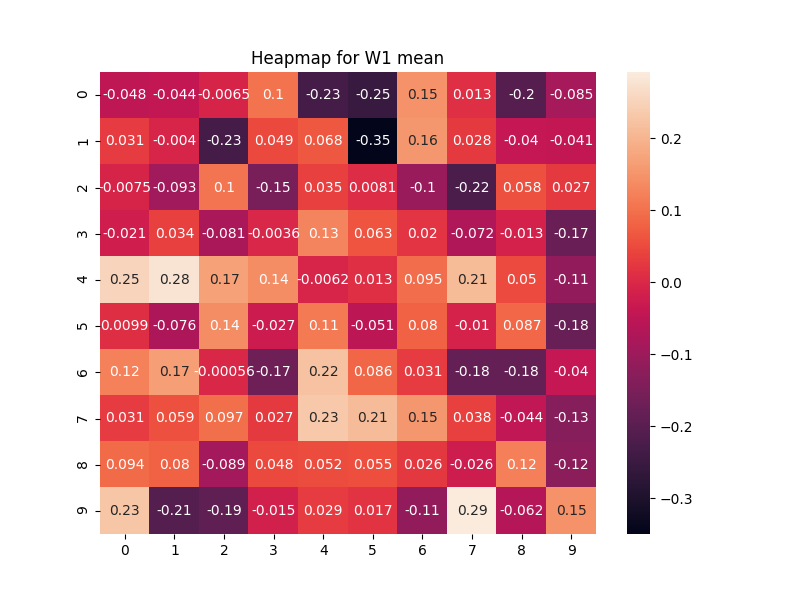
\includegraphics[width=0.5\textwidth]{../figs/4_daphne_w1_mean_heatmap.png}%
        \label{fig:a}%
        }%
    \hfill%
    \subfloat[Samples from the posterior for bias]{%
        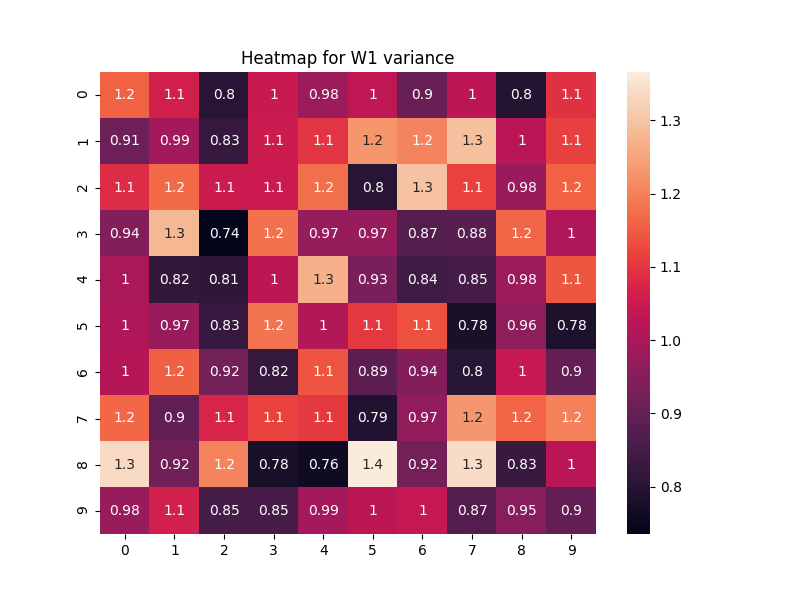
\includegraphics[width=0.5\textwidth]{../figs/4_daphne_w1_variance_heatmap.png}%%
        \label{fig:b}%
        }%
        \caption{Posterior distribution for slope and bias for 4.daphne using Black Box Variational Inference}
\end{figure}

\begin{figure}[!htp] 
    \centering
    \subfloat[Samples from the posterior for slope]{%
        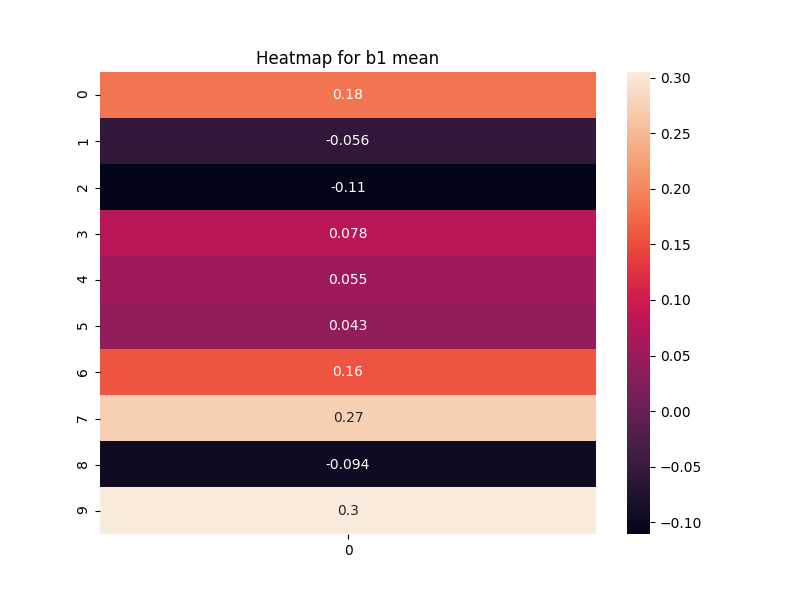
\includegraphics[width=0.5\textwidth]{../figs/4_daphne_b1_mean_heatmap.png}%
        \label{fig:a}%
        }%
    \hfill%
    \subfloat[Samples from the posterior for bias]{%
        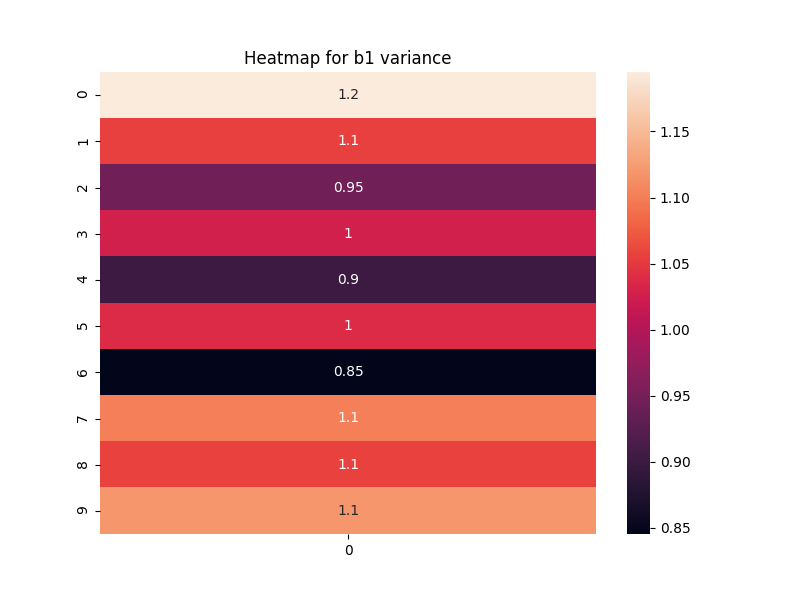
\includegraphics[width=0.5\textwidth]{../figs/4_daphne_b1_variance_heatmap.png}%%
        \label{fig:b}%
        }%
        \caption{Posterior distribution for slope and bias for 4.daphne using Black Box Variational Inference}
\end{figure}



\end{enumerate}
\end{document}